% =============================================================
%  Plan 08 — Learned Memory Wrapper
%  Architecture diagram, version: v1.5 (2026-06-05)
%  v1.5 = v0/v1 recurrent mem-X wrapper + INTRINSIC-SIGNAL DO-NO-HARM GATE.
%
%  Compile: pdflatex architecture-v1.5.tex   (tikz, positioning, fit,
%           shapes.geometric, arrows.meta, calc, decorations.pathreplacing, backgrounds)
% =============================================================
\documentclass[border=12pt,tikz]{standalone}
\usepackage{tikz}
\usepackage{amsmath,amssymb}
\usetikzlibrary{positioning,fit,shapes.geometric,arrows.meta,calc,
                decorations.pathreplacing,backgrounds}

\definecolor{frozenfill}{HTML}{E8ECEF}     % grey  — frozen (no grad)
\definecolor{trainedfill}{HTML}{FFE6B3}    % amber — trainable
\definecolor{datafill}{HTML}{D8E8FB}       % blue  — data / state
\definecolor{probefill}{HTML}{E7F5E1}      % green — probes / signals
\definecolor{gatefill}{HTML}{F6C9C0}       % red   — the NEW gate (v1.5)
\definecolor{arrowclr}{HTML}{2B2B2B}

\tikzset{
  block/.style   = {draw, rounded corners=2pt, minimum height=8mm, inner sep=4pt, align=center, font=\small},
  frozen/.style  = {block, fill=frozenfill},
  trained/.style = {block, fill=trainedfill, very thick},
  data/.style    = {block, fill=datafill},
  probe/.style   = {block, fill=probefill, dashed, font=\footnotesize},
  gate/.style    = {block, fill=gatefill, very thick, draw=red!55!black},
  flow/.style    = {-Latex, thick, draw=arrowclr},
  fback/.style   = {-Latex, thick, dashed, draw=arrowclr!70},
  sig/.style     = {-Latex, thick, draw=red!55!black},
}

\begin{document}
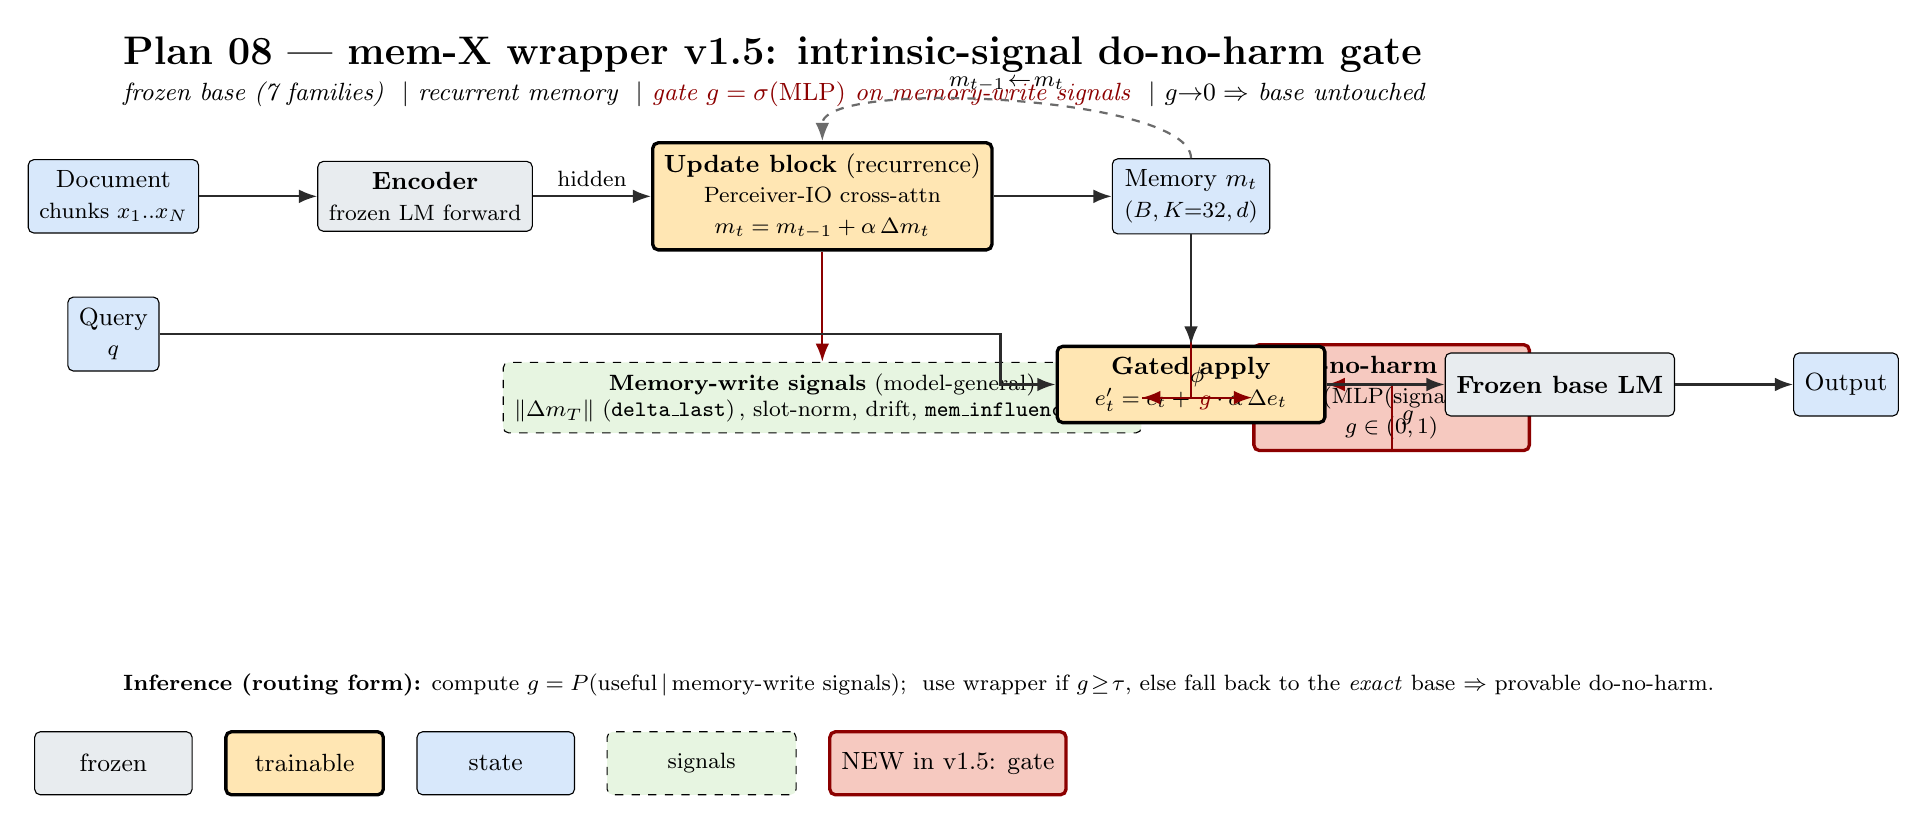
\begin{tikzpicture}[node distance=8mm and 15mm]

\node[font=\Large\bfseries, anchor=west] (title) at (0,5.0)
  {Plan 08 — mem-X wrapper \textbf{v1.5}: intrinsic-signal do-no-harm gate};
\node[font=\small\itshape, anchor=west] (sub) at (0,4.5)
  {frozen base (7 families) \ $|$\ recurrent memory \ $|$\ \textcolor{red!55!black}{gate $g=\sigma(\mathrm{MLP})$ on memory-write signals} \ $|$\ $g{\to}0\Rightarrow$ base untouched};

%% input
\node[data]                         (doc) at (0,3.2) {Document\\\footnotesize chunks $x_1..x_N$};
\node[data, below=of doc]           (qry) {Query\\\footnotesize $q$};

%% encoder + recurrence
\node[frozen, right=of doc]         (enc) {\textbf{Encoder}\\\footnotesize frozen LM forward};
\node[trained, right=of enc, minimum width=42mm] (upd)
  {\textbf{Update block} (recurrence)\\\footnotesize Perceiver-IO cross-attn\\\footnotesize $m_t=m_{t-1}+\alpha\,\Delta m_t$};
\node[data, right=of upd, minimum width=20mm] (mem) {Memory $m_t$\\\footnotesize $(B,K{=}32,d)$};

%% memory-write signals -> gate  (the v1.5 addition)
\node[probe, below=14mm of upd, minimum width=46mm] (sig)
  {\textbf{Memory-write signals} (model-general)\\\footnotesize $\|\Delta m_T\|$ (\texttt{delta\_last})\,,\ slot-norm,\ drift,\ \texttt{mem\_influence\_span}};
\node[gate, right=14mm of sig, minimum width=30mm] (gate)
  {\textbf{Do-no-harm gate}\\\footnotesize $g=\sigma(\mathrm{MLP}(\text{signals}\,[,q]))$\\\footnotesize $g\in(0,1)$};

%% apply + base
\node[trained, below=14mm of mem, minimum width=34mm] (apply)
  {\textbf{Gated apply}\\\footnotesize $e'_t=e_t+\,\textcolor{red!55!black}{g}\cdot\alpha\,\Delta e_t$};
\node[frozen, right=of apply, minimum width=28mm] (base) {\textbf{Frozen base LM}};
\node[data, right=of base]          (out) {Output};

%% flows
\draw[flow] (doc) -- (enc);
\draw[flow] (enc) -- node[above,font=\footnotesize]{hidden} (upd);
\draw[flow] (upd) -- (mem);
\draw[fback] (mem.north) .. controls +(0,8mm) and +(0,8mm) .. (upd.north)
  node[midway,above,font=\footnotesize]{$m_{t-1}\!\leftarrow\!m_t$};
\draw[sig] (upd.south) -- (sig.north);
\draw[sig] (mem.south) |- (sig.east);
\draw[sig] (sig) -- node[above,font=\footnotesize]{$\phi$} (gate);
\draw[sig] (gate.south) |- node[pos=0.25,right,font=\footnotesize]{$g$} (apply.east);
\draw[flow] (mem.south) -- (apply.north);
\draw[flow] (qry.east) -| ($(apply.west)+(-7mm,0)$) -- (apply.west);
\draw[flow] (apply) -- (base);
\draw[flow] (base) -- (out);

%% inference routing note
\node[font=\footnotesize, align=left, anchor=west] at (0,-3.0)
  {\textbf{Inference (routing form):} compute $g=P(\text{useful}\,|\,\text{memory-write signals})$;\ \ use wrapper if $g\!\ge\!\tau$, else fall back to the \emph{exact} base $\Rightarrow$ provable do-no-harm.};

%% legend
\begin{scope}[shift={(0,-4.0)}, font=\footnotesize]
  \node[frozen, minimum width=20mm] (l1) {frozen};
  \node[trained, right=4mm of l1, minimum width=20mm] (l2) {trainable};
  \node[data, right=4mm of l2, minimum width=20mm] (l3) {state};
  \node[probe, right=4mm of l3, minimum width=24mm] (l4) {signals};
  \node[gate, right=4mm of l4, minimum width=30mm] (l5) {NEW in v1.5: gate};
\end{scope}

\end{tikzpicture}
\end{document}
